\section{Модел с няколко местообитания}
\begin{frame}[t]{Многомерен модел на Bichara}
  Допускания на модела:
  \begin{enumerate}
    \item Има $m$ области, които се обитават от комари и $n$ популации хора, които ги посещават.
    \item Комарите не се движат между областите.
    \item Всяка от групите хора и комари е от константен брой.
    \item Мобилността на хората в различните местообитания е константна.
    \item Честотата на ухапвания на комари за всяка област е константна.
    \item Хората могат да оздравеят, а комарите - не.
  \end{enumerate}
\end{frame}

\begin{frame}[t]{Многомерен модел на Bichara. Означения}
  \begin{enumerate}
    \item $X_i(t)$ е броя заразени с малария хора в момент $t$, $i=\overline{1,n}$.
    \item $Y_j(t)$ е броя заразени с малария комари в момент $t$, $j=\overline{1,m}$.
    \item $N_i$ е броя хора, а $M_j$ е броя комари за съответните групи.
    \item $\gamma_i$ са скорости на оздравяване на хората.
    \item $\mu_j$ са скорости на смъртност на комарите.
    \item $a_j$ е честотата на ухапване на комарите за единица време.
    \item $\beta_{vh}$ вероятност за предаване комар->човек, а $\beta_{hv}$ - човек->комар.
    \item $p_{ij}$ - средна вероятност човек от $i$ да е в $j$.
  \end{enumerate}
\end{frame}

\begin{frame}[t]{Многомерен модел на Bichara. Уравнение за контактите}
  Средния брой ухапвания на комари в съответните области по техния брой трябва да е същия като средния брой ухапвания на хора от популации по броя им в съответната област, сумирайки по всяка попилация.
  \begin{equation}
    a_j M_j = b_j \sum_{i=1}^n p_{ij} N_i \iff b_j = \frac{a_j M_j}{\sum_{i=1}^n p_{ij} N_i}
  \end{equation}
  При направените допускания, в момент $t$, в местообитание $j$ съотношението на заразени към всички хора е:
  \begin{equation}
    \frac{\sum_{i=1}^n p_{ij} X_i(t)}{\sum_{i=1}^n p_{ij} N_i}
  \end{equation}
  Аналогично на модела на Ross може да получим:
\end{frame}

\begin{frame}[t]{Многомерен модел на Bichara. Извеждане}
  В момент $t$ заразените хора $X_i$ се увеличават от ухапване на незаразен човек от $i$ заразени комари в различните местообитания $j$, а намаляват пропорционално на броя си с коефициента на оздравяване.
  
  Достига се до $\dot{X}_i(t) = \sum_{j=1}^{m} \beta_{vh} b_j p_{ij} (N_i - X_i(t)) \frac{I_j}{M_j} - \gamma_i X_i(t)$.
\end{frame}

\begin{frame}[t]{Многомерен модел на Bichara. Извеждане}
  В момент $t$ заразените комари $Y_j$ се увеличават от ухапване на заразен човек от някое от различните местообитания $i$ от незаразен комар в местообитание $j$, а намаляват пропорционално на броя си с коефициента на смъртност.
  
  Достига се до $\dot{Y}_j(t) = \beta_{hv} a_j (M_j - Y_j(t)) \frac{\sum_{i=1}^n p_{ij} X_i(t)}{\sum_{i=1}^n p_{ij} N_i} - \mu_j Y_j(t)$.
\end{frame}

\begin{frame}[t]{Многомерен модел на Bichara. Краен вид}
  \begin{equation}
    \label{eq:MigrationProblem}
    \begin{split}
      &\dot{X}_i(t) = \beta_{vh} (N_i - X_i(t)) \sum_{j=1}^{m} \frac{p_{ij} a_j I_j}{\sum_{k=1}^n p_{kj} N_k} - \gamma_i X_i(t), \quad i=\overline{1, n} \\
      &\dot{Y}_j(t) = \beta_{hv} a_j (M_j - Y(t)) \frac{\sum_{i=1}^n p_{ij} X_i(t)}{\sum_{i=1}^n p_{ij} N_i} - \mu_j Y_j(t), \quad j=\overline{1, m}
    \end{split}
  \end{equation}
  С помощта на теорията на кооперативните системи може да се докаже:
  \begin{proposition}
    За системата \ref{eq:MigrationProblem} е в сила точно едно от:
    \begin{enumerate}
      \item $\mathscr{R}_0 \leq 1$ и $\boldsymbol{0}$ е единствената равновесна точка и е глобално асимптотично устойчива.
      \item $\mathscr{R}_0 > 1$ и $\boldsymbol{0}$ е неустойчива равновесна точка, като ако системата е неразложима, има друга равновесна глобално асимптотично устойчива точка.
    \end{enumerate}
  \end{proposition}
\end{frame}

\begin{frame}[t]{Резултати на Bichara}
  \begin{figure}[h]
    \centering
    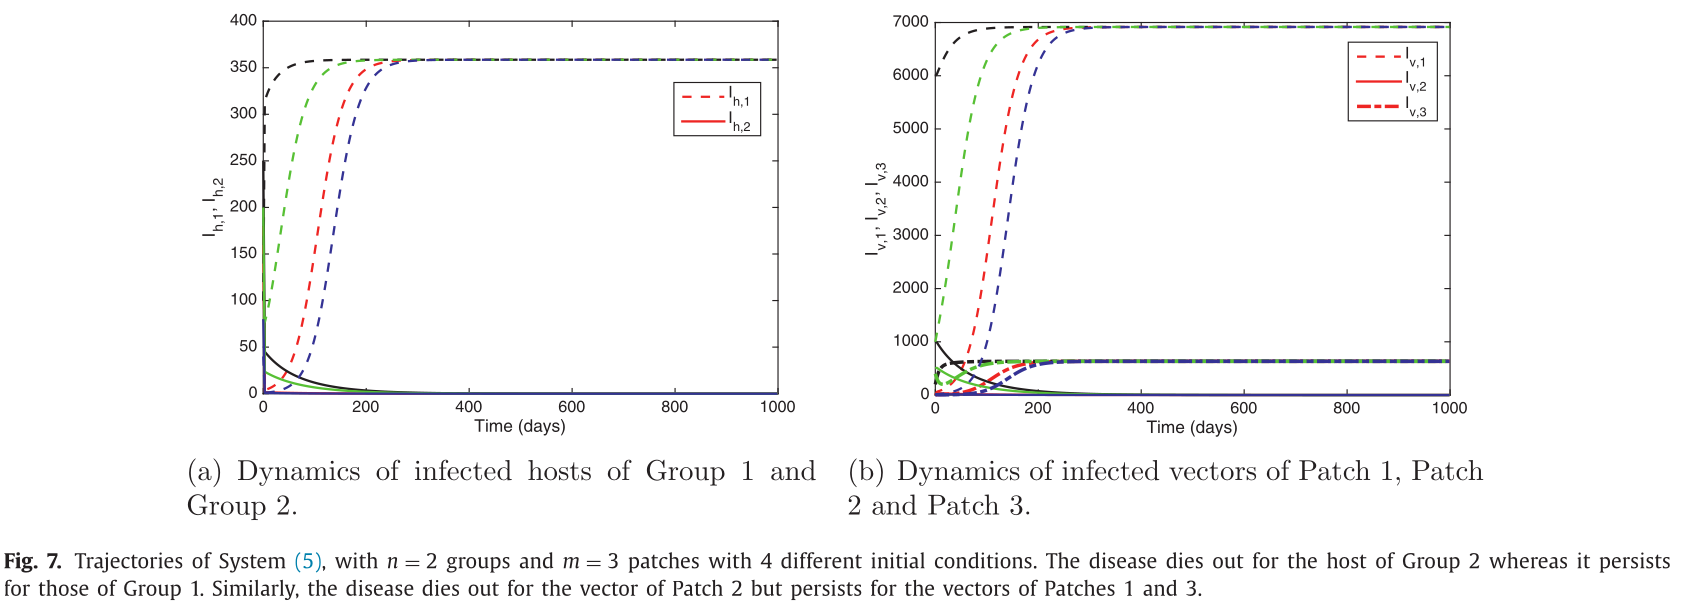
\includegraphics[width=0.95\paperwidth, height=0.65\paperheight]{bichara-interesting-result.png}
    \caption{Сложно развитие на малария}
  \end{figure}
\end{frame}
